\providecommand{\main}{../../../..}
\documentclass[\main/dresen_thesis.tex]{subfiles}
\begin{document}
  \label{sec:doublelayers:layers:sem}

  \begin{figure}[tb]
    \centering
    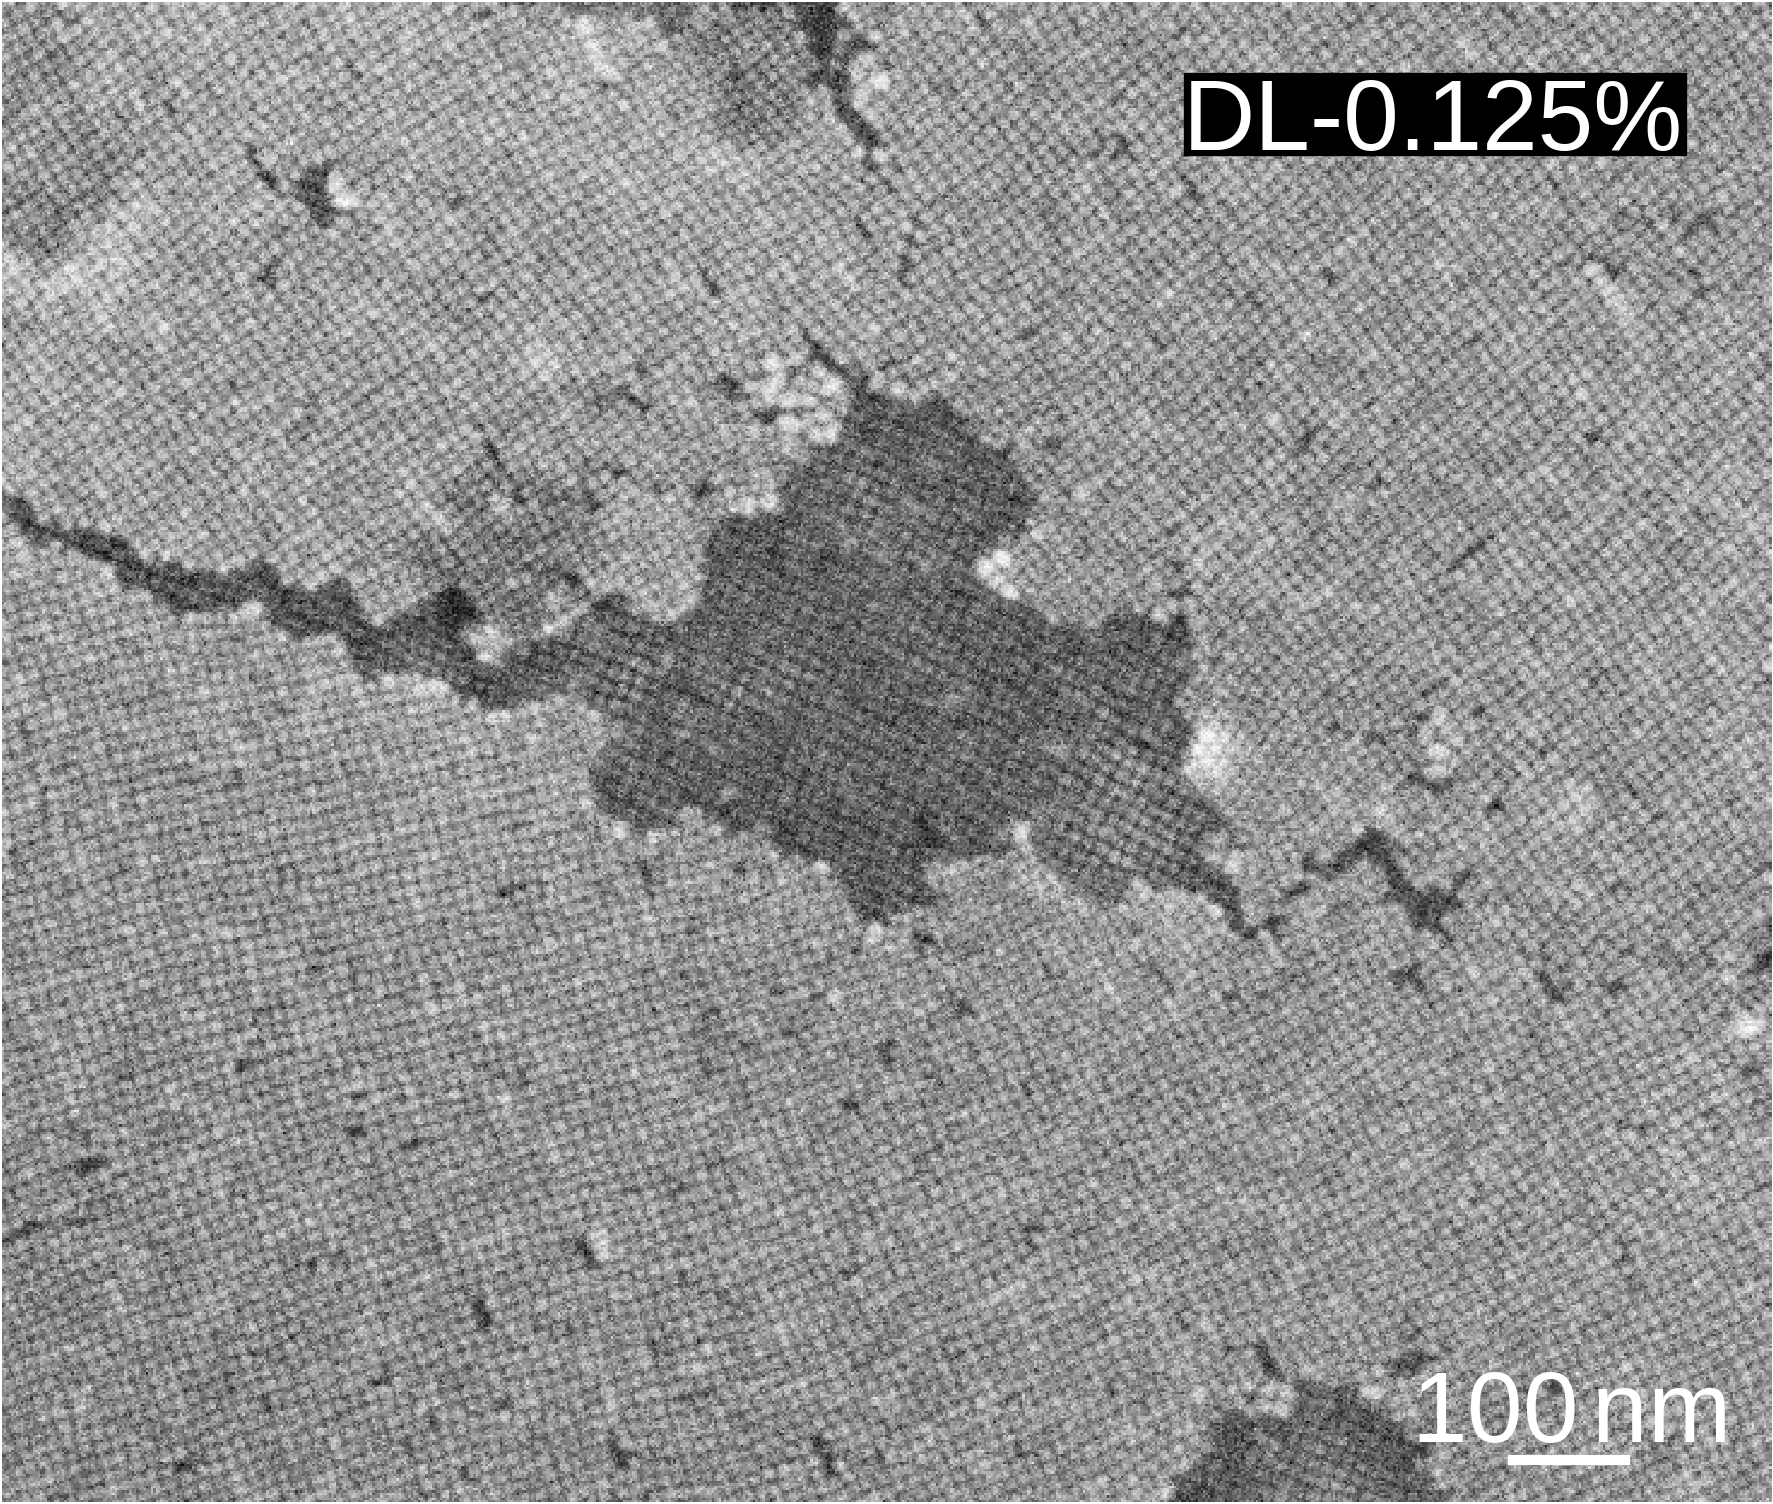
\includegraphics{doubleLayers_SEM_DL-0_125}
    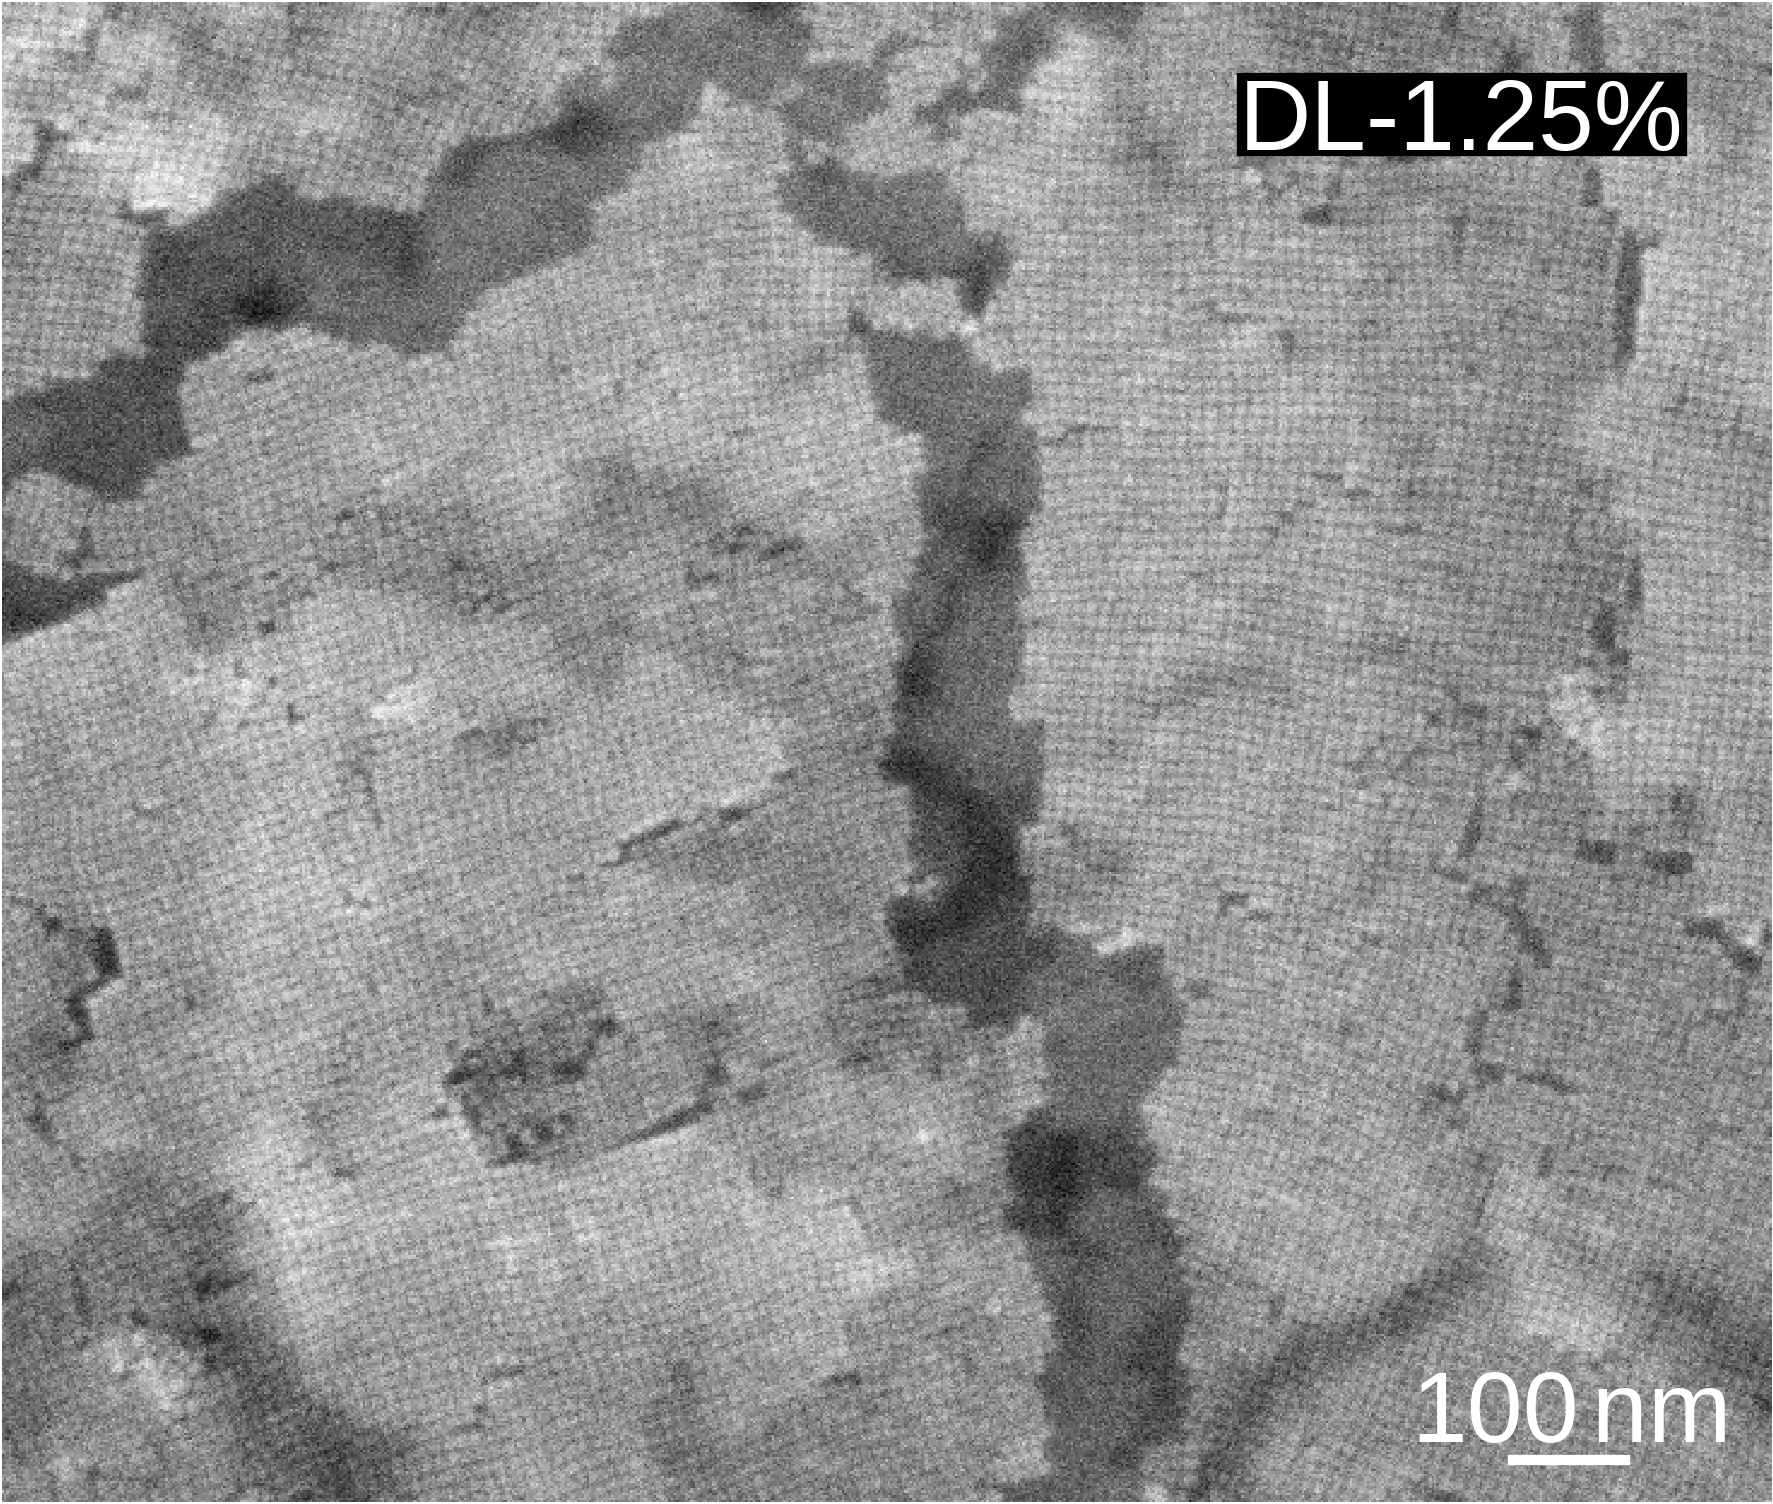
\includegraphics{doubleLayers_SEM_DL-1_25}
    \caption{\label{fig:doublelayers:layers:sem}Top view SEM micrographs of DL-0.125\% (left) and DL-1.25\% (right).}
  \end{figure}

  An initial evaluation of the double layers is obtained from top view micrographs, shown exemplary in \reffig{fig:doublelayers:layers:sem}.
  The square lattice ordering of the top layer is observable in all cases and additionally it is possible to spot the lower layer by looking through gaps in the structure.
  For the samples, which were prepared with spacer layers from low concentrated PMMA dispersions, the lower layer is clearly visible in the top view micrograph, whereas it is less visible for samples prepared with higher concentrated PMMA dispersions.

  The cross-sectional views of five double layer samples prepared with varied PMMA concentration during spin-coating are shown in \reffig{fig:doublelayers:layers:xs} and reveal the thickness of the spacer layers.
  Measuring the distance from the wafer surface to the top of the upper layer, the sample thickness is estimated at multiple positions of the SEM micrographs, which is additionally shown with respect to the PMMA concentration.
  Additionally marked with a black line is the thickness of two cube edge lengths, neglecting the oleic acid shell, which shows the lower limit for a double layer sample of Ac-CoFe-C.
  An approximately linear dependence between the concentration and thickness is visible from the observed thickness with the relation
  \begin{align}
    \frac{D_\mathrm{sample}}{\unit{nm}} \eq 56(5) \frac{c_V^\mathrm{PMMA}}{\%}  + 14(8).
  \end{align}

  From the SEM images, the two samples prepared by $0.125 \%$ and $0.25\%$ show no significant PMMA layer and are close to the thickness expected from two nanocubes and additional oleic acid surfactant.
  Above this, the PMMA layer is well visible in SEM and the observed linear dependence alludes that the spin coating process is capable to precisely tune the thickness to any desired value by setting the PMMA concentration.

  \begin{figure}[tb]
    \centering
    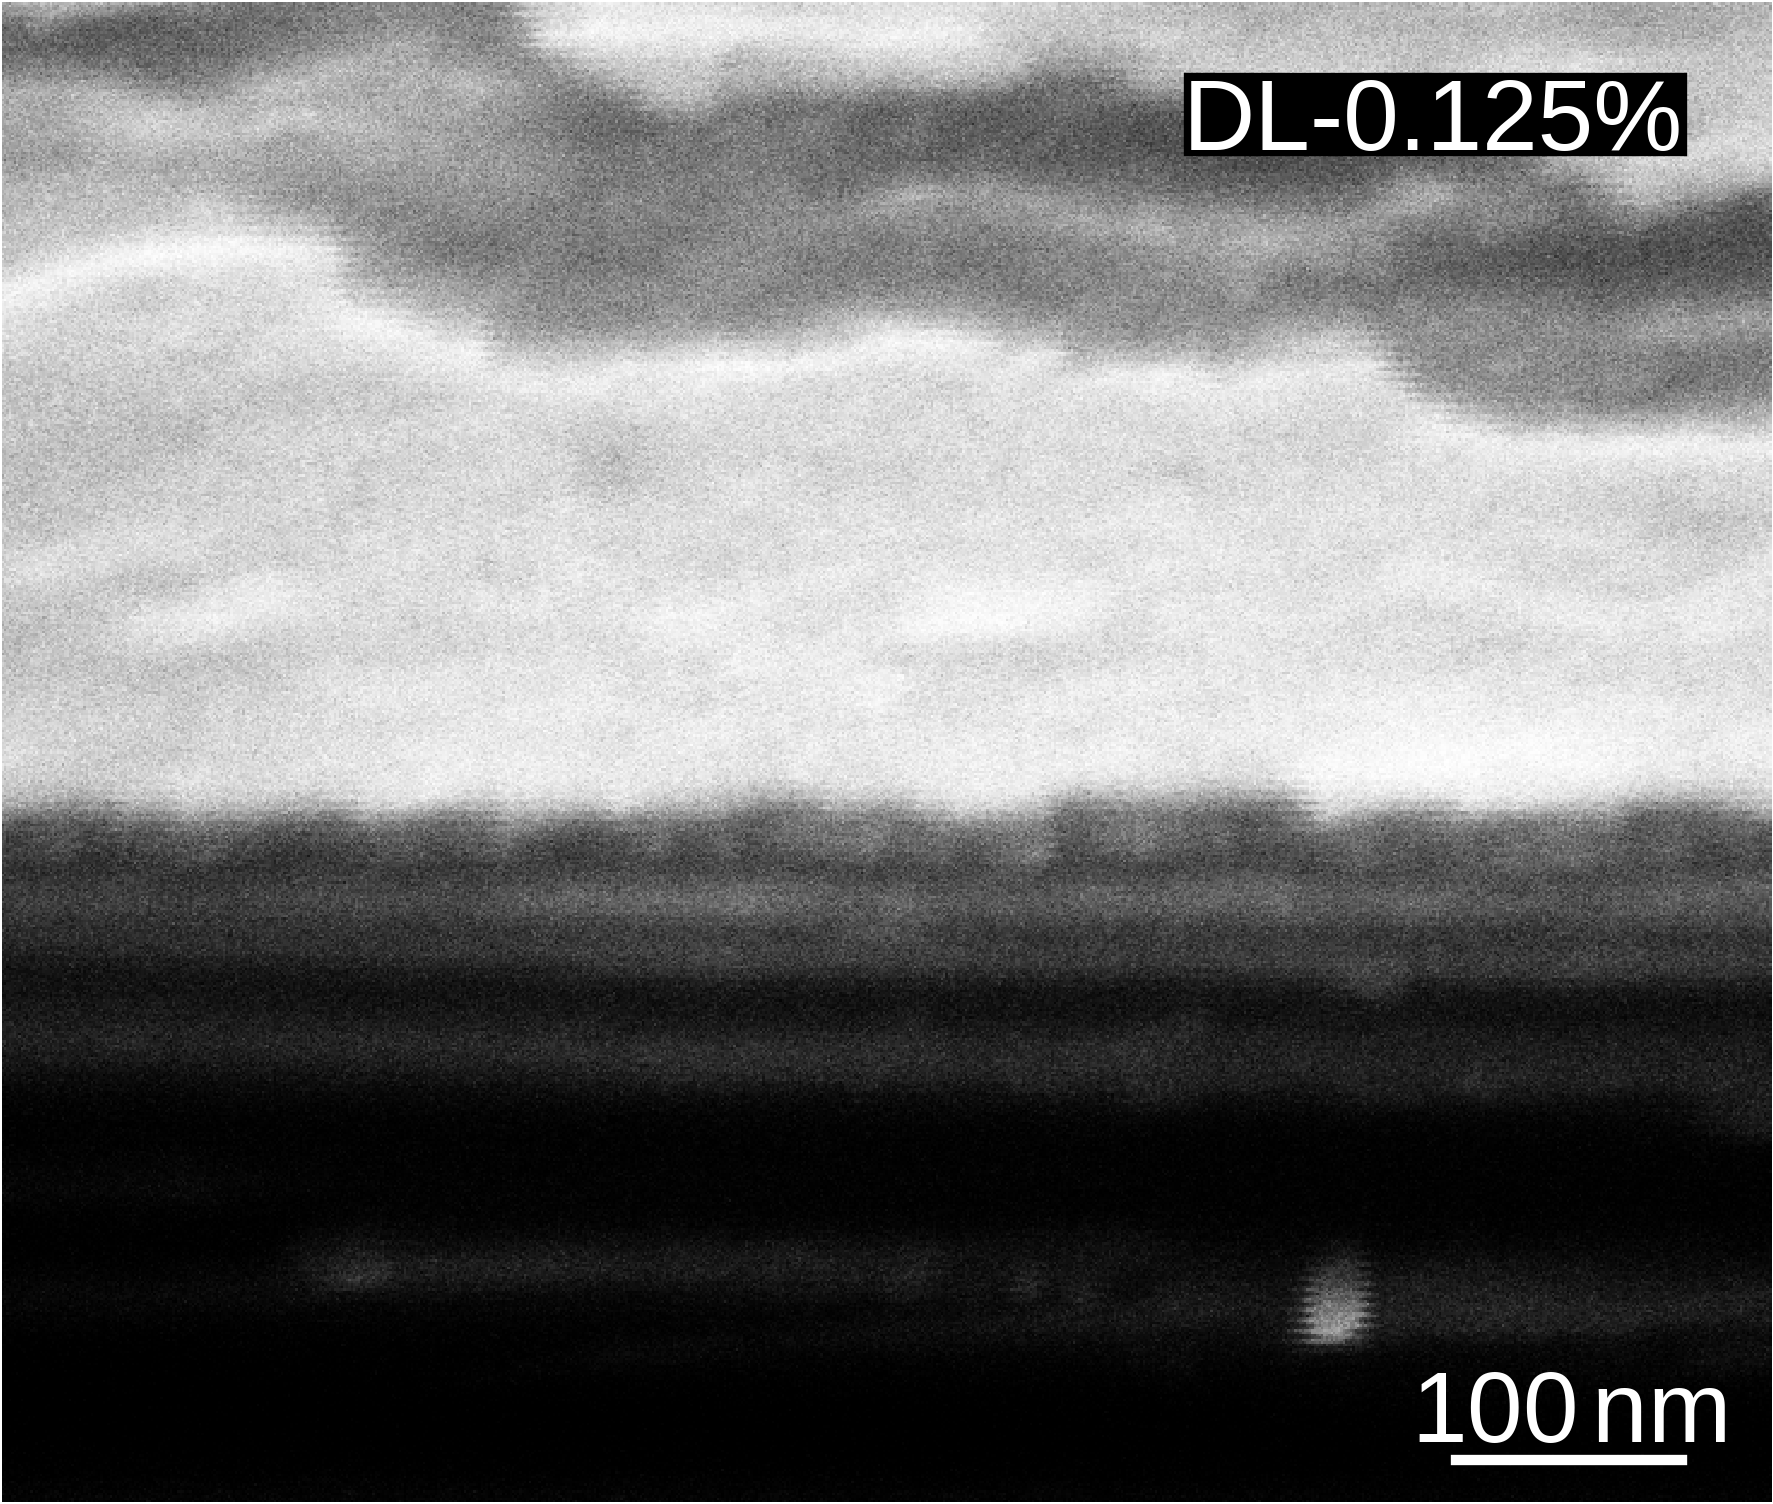
\includegraphics{doubleLayers_SEMxs_DL-0_125}
    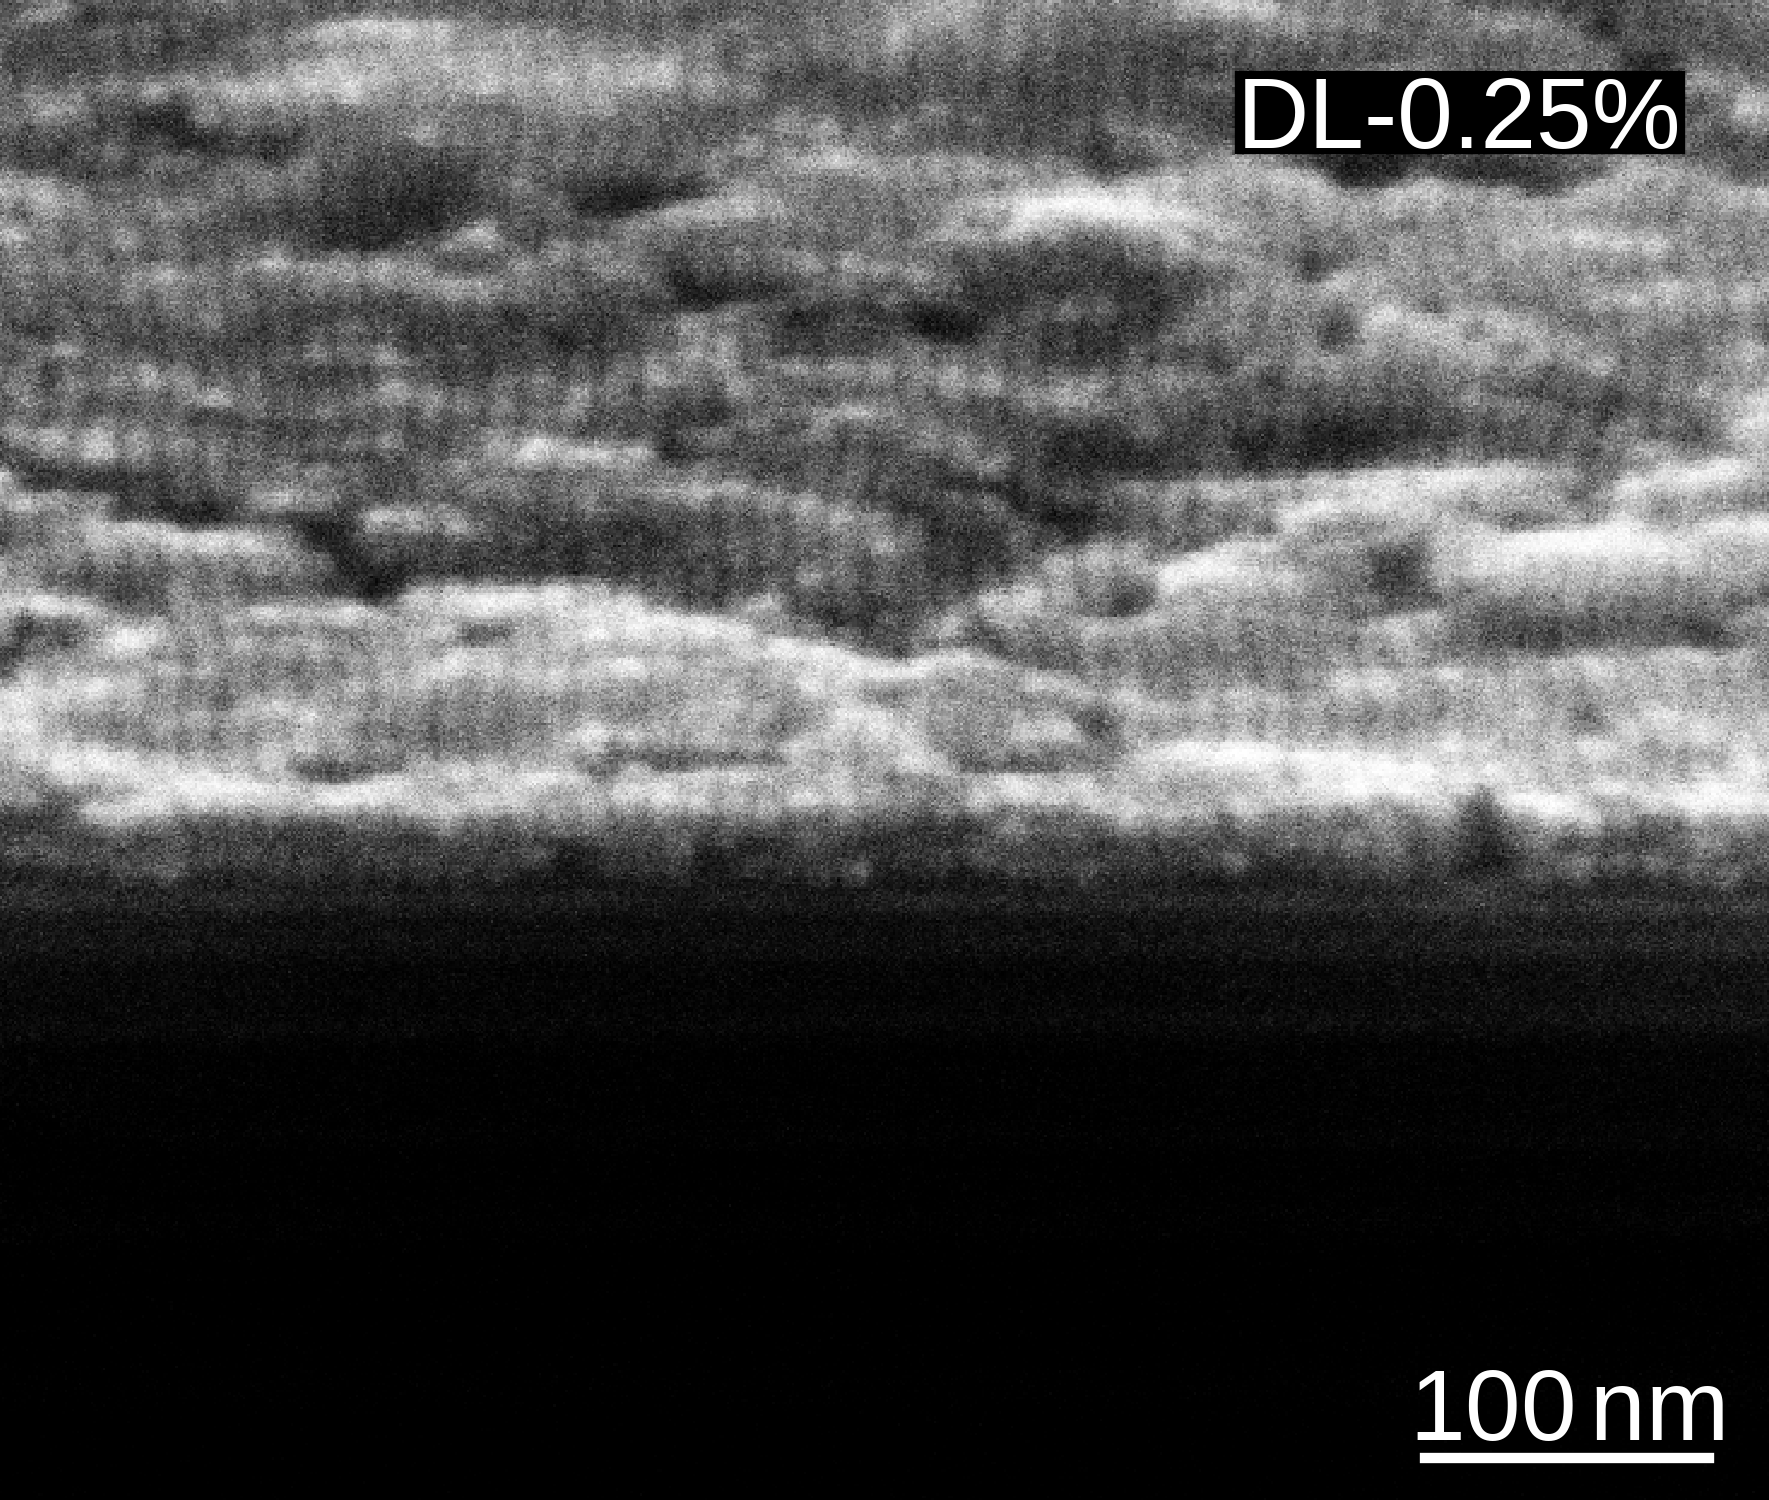
\includegraphics{doubleLayers_SEMxs_DL-0_25}
    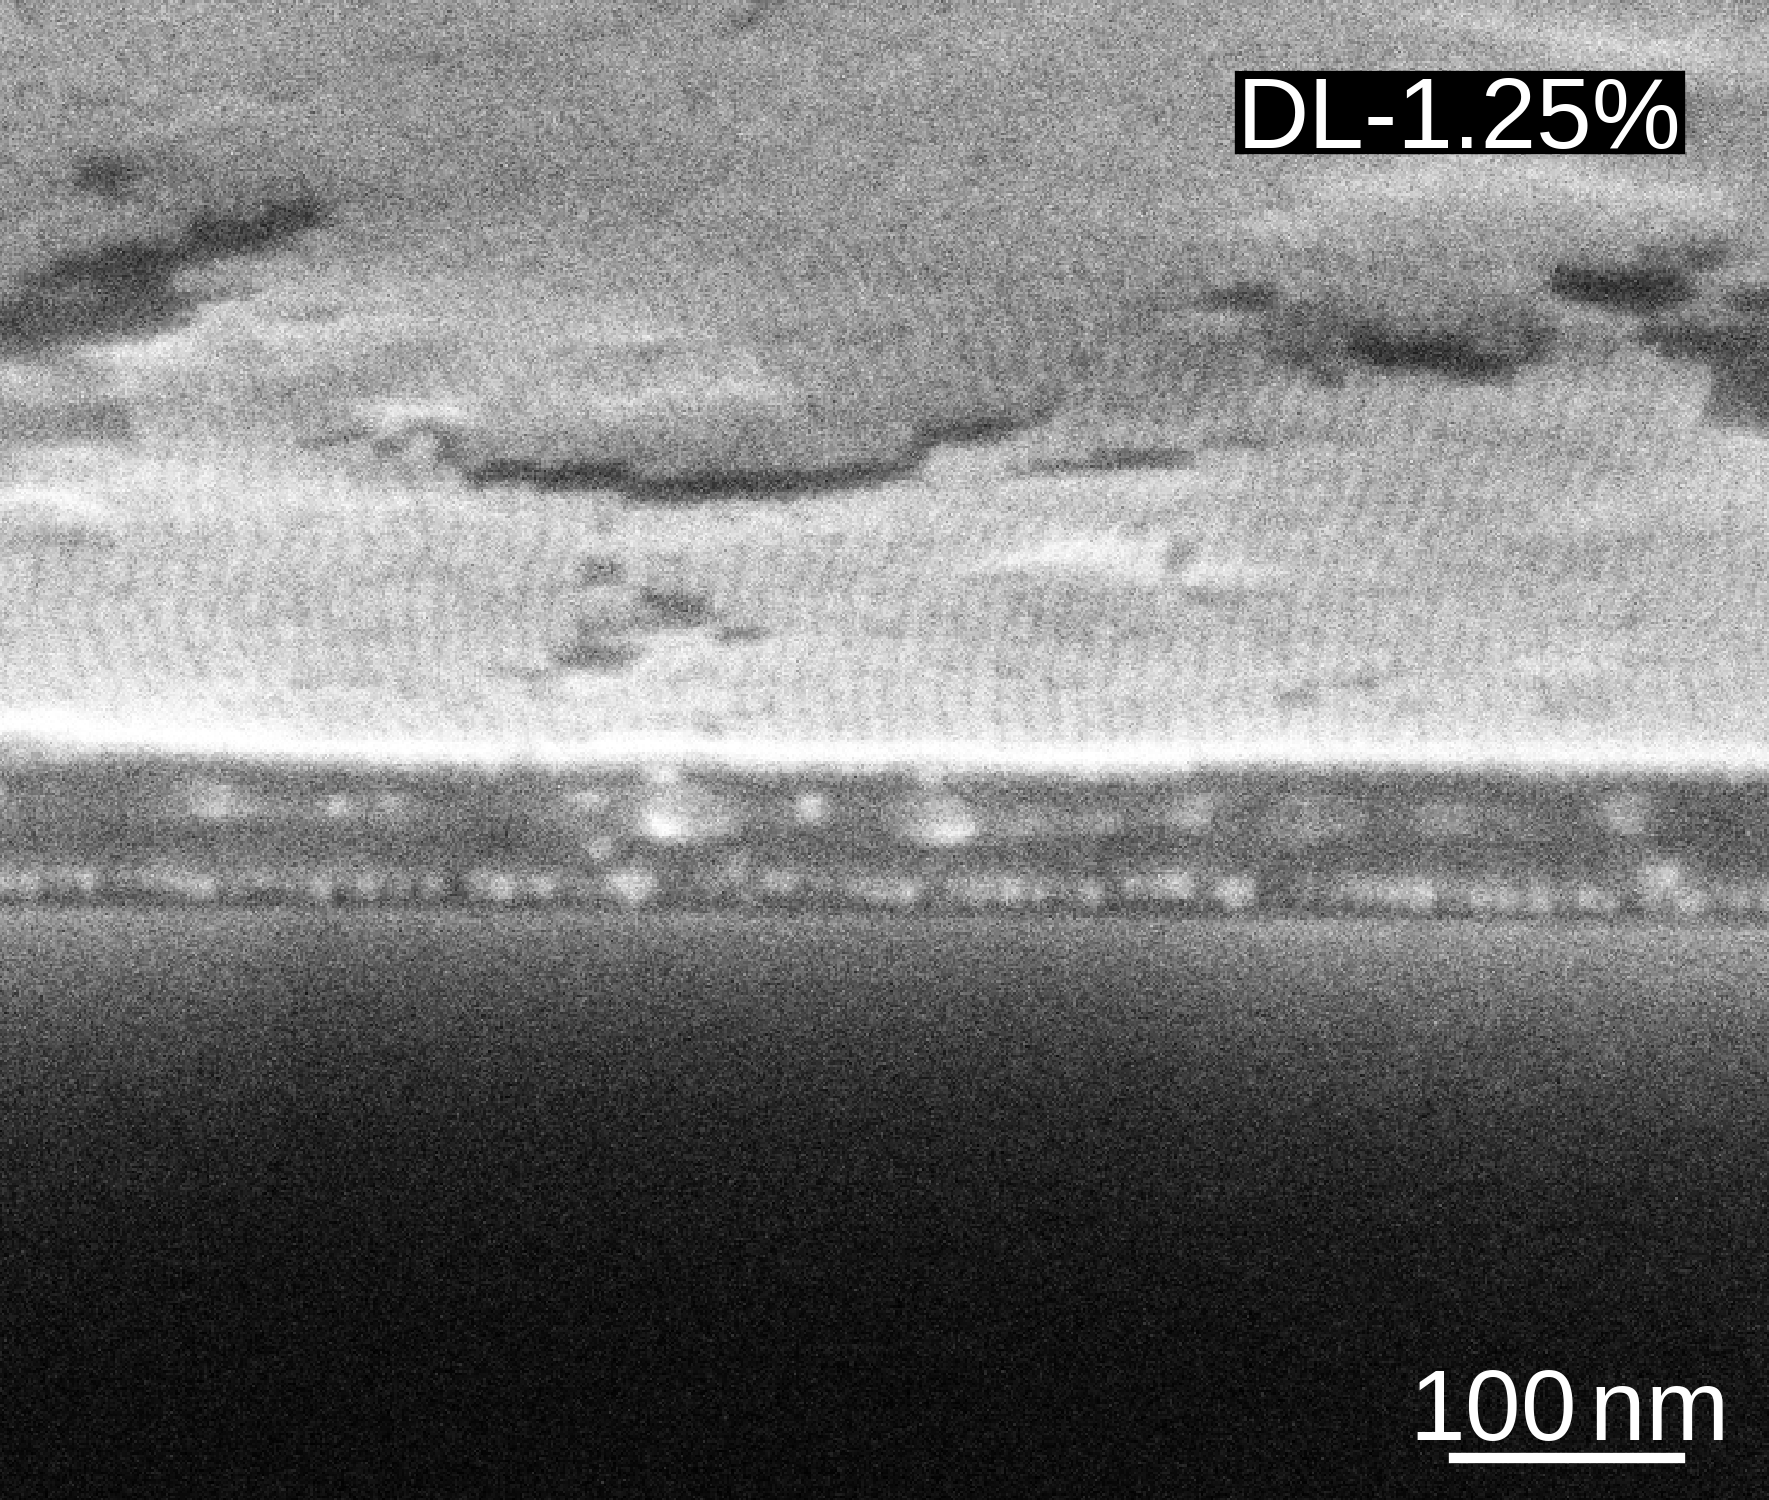
\includegraphics{doubleLayers_SEMxs_DL-1_25}
    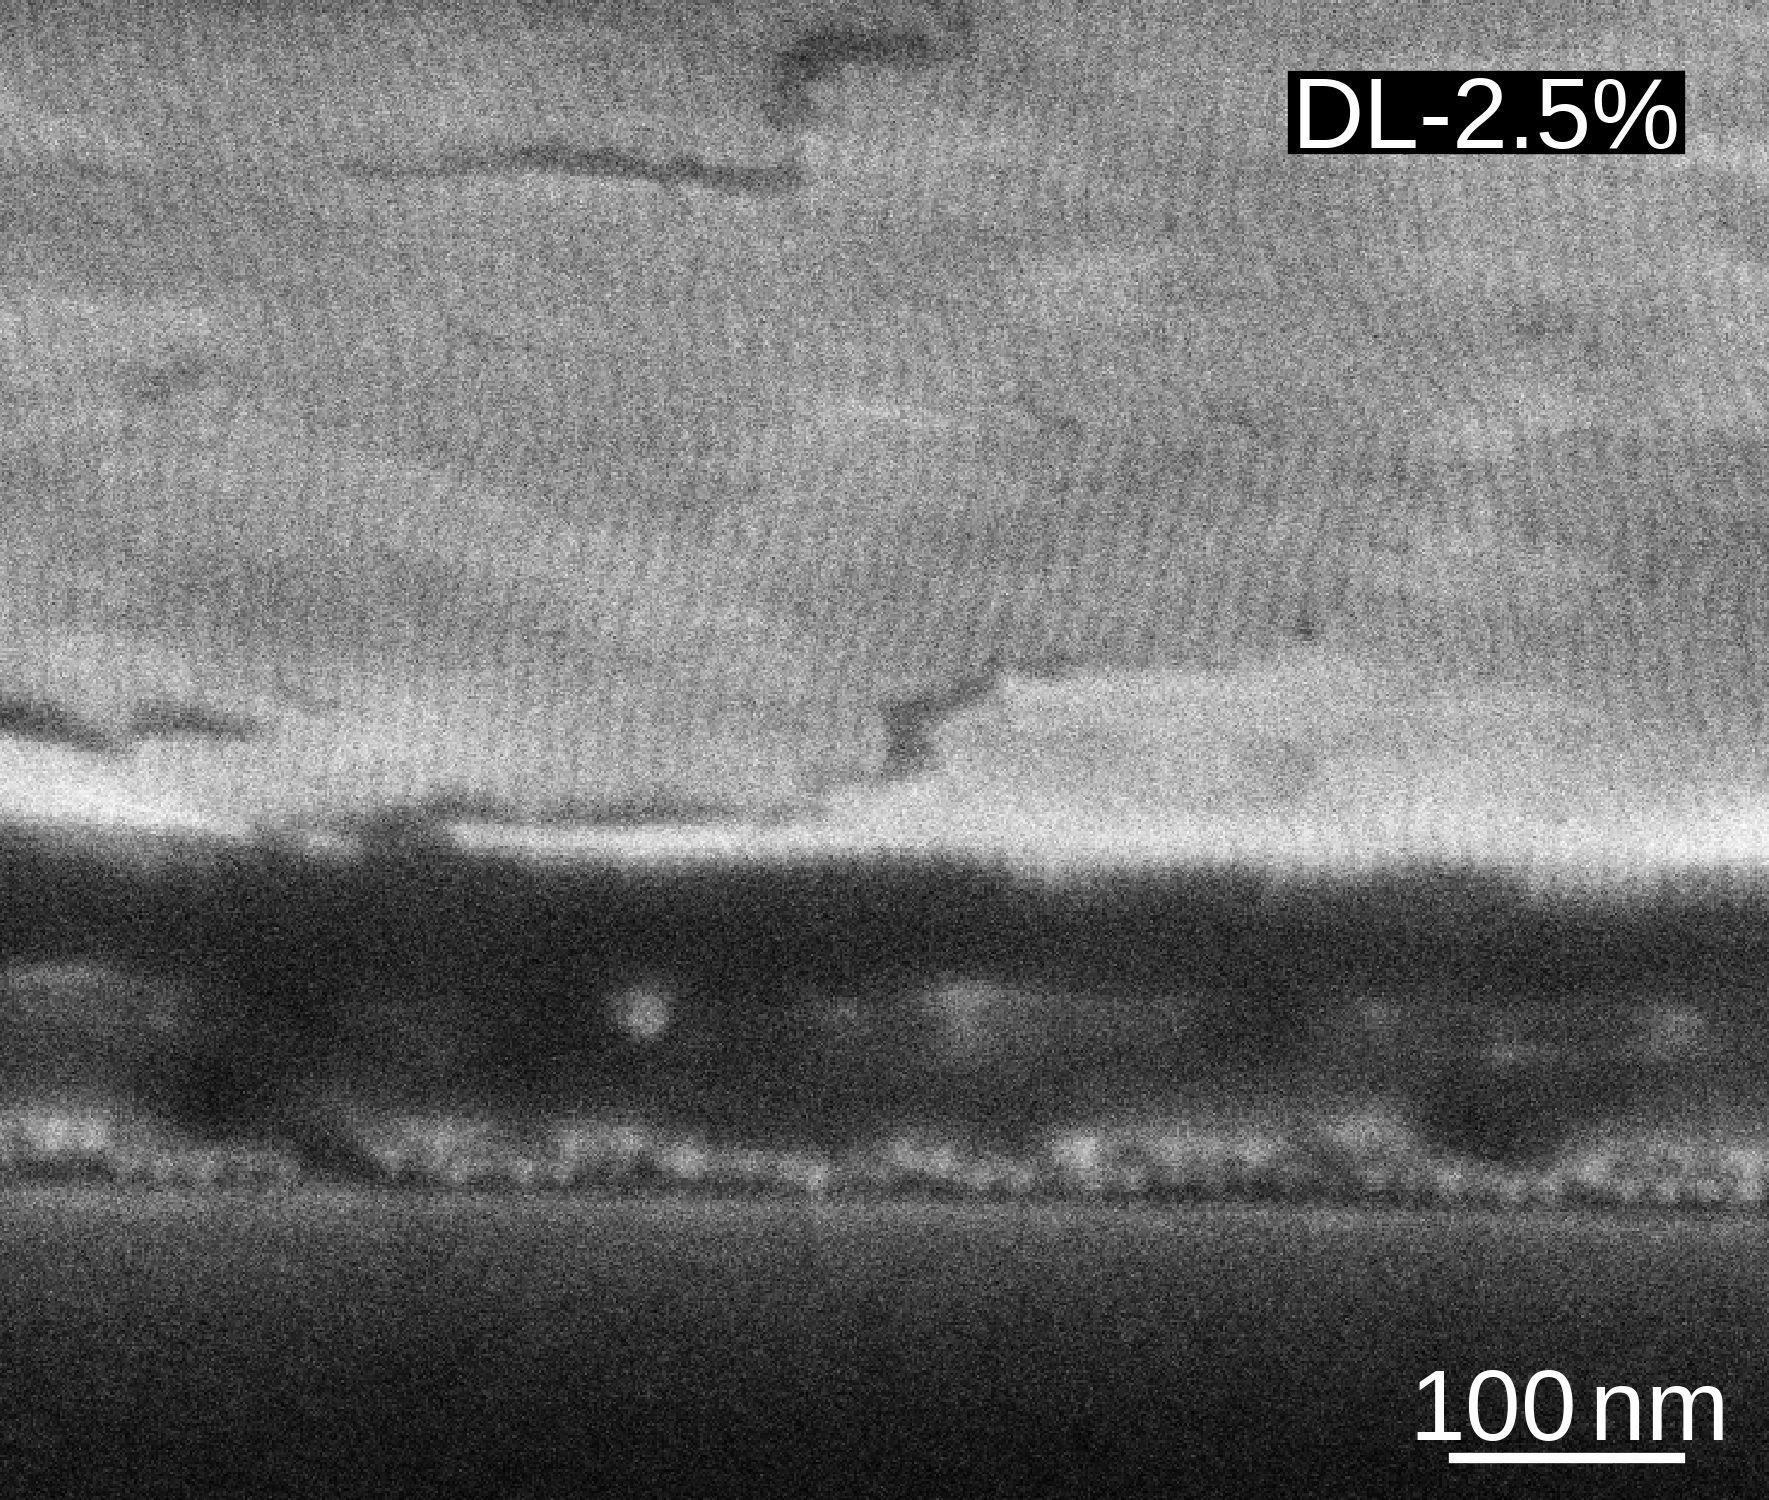
\includegraphics{doubleLayers_SEMxs_DL-2_5}
    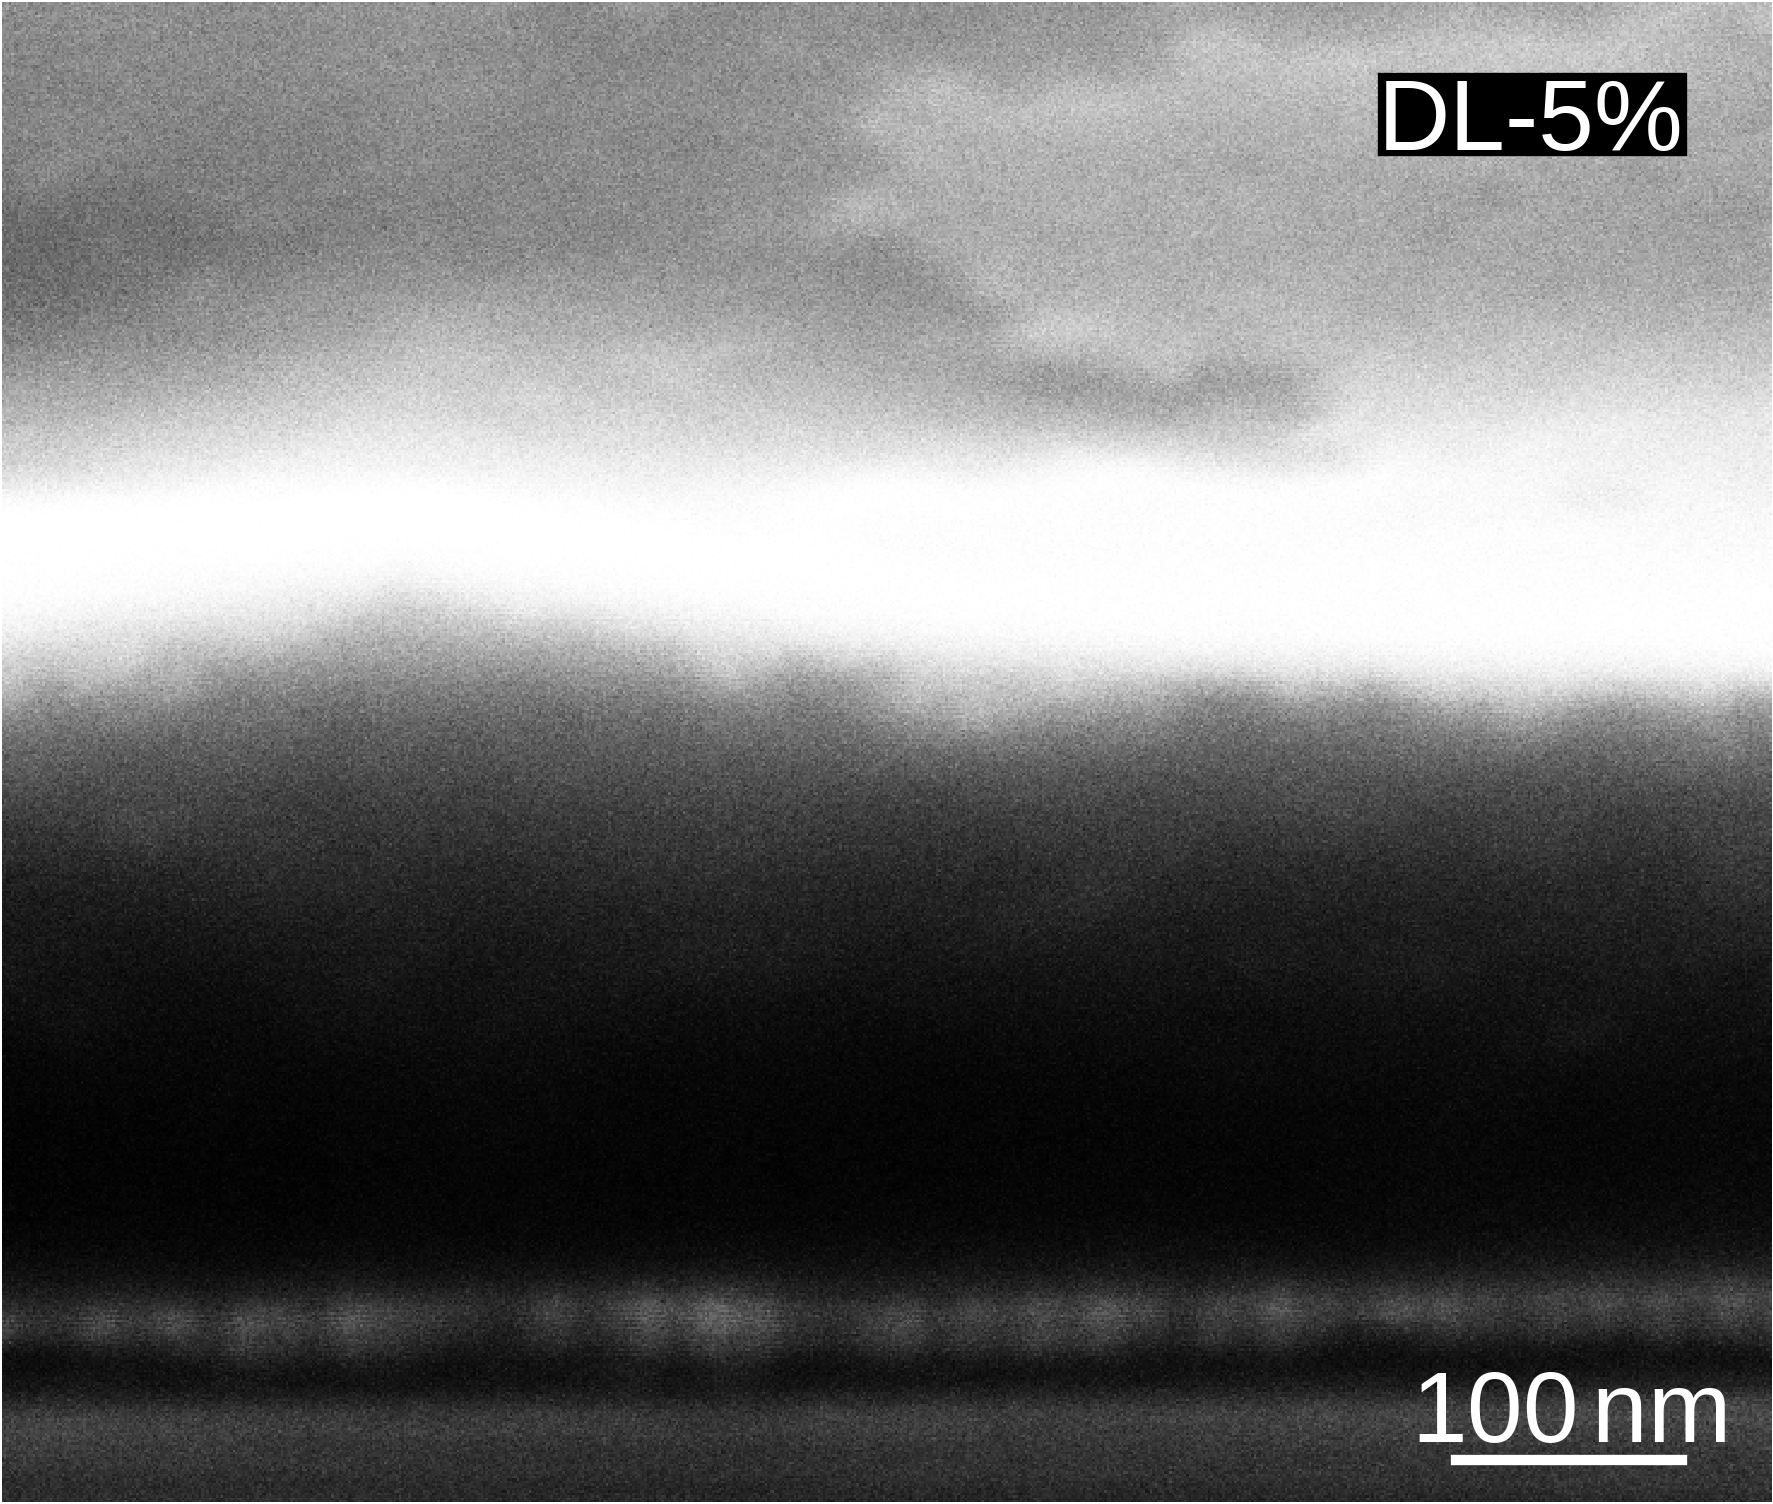
\includegraphics{doubleLayers_SEMxs_DL-5}
    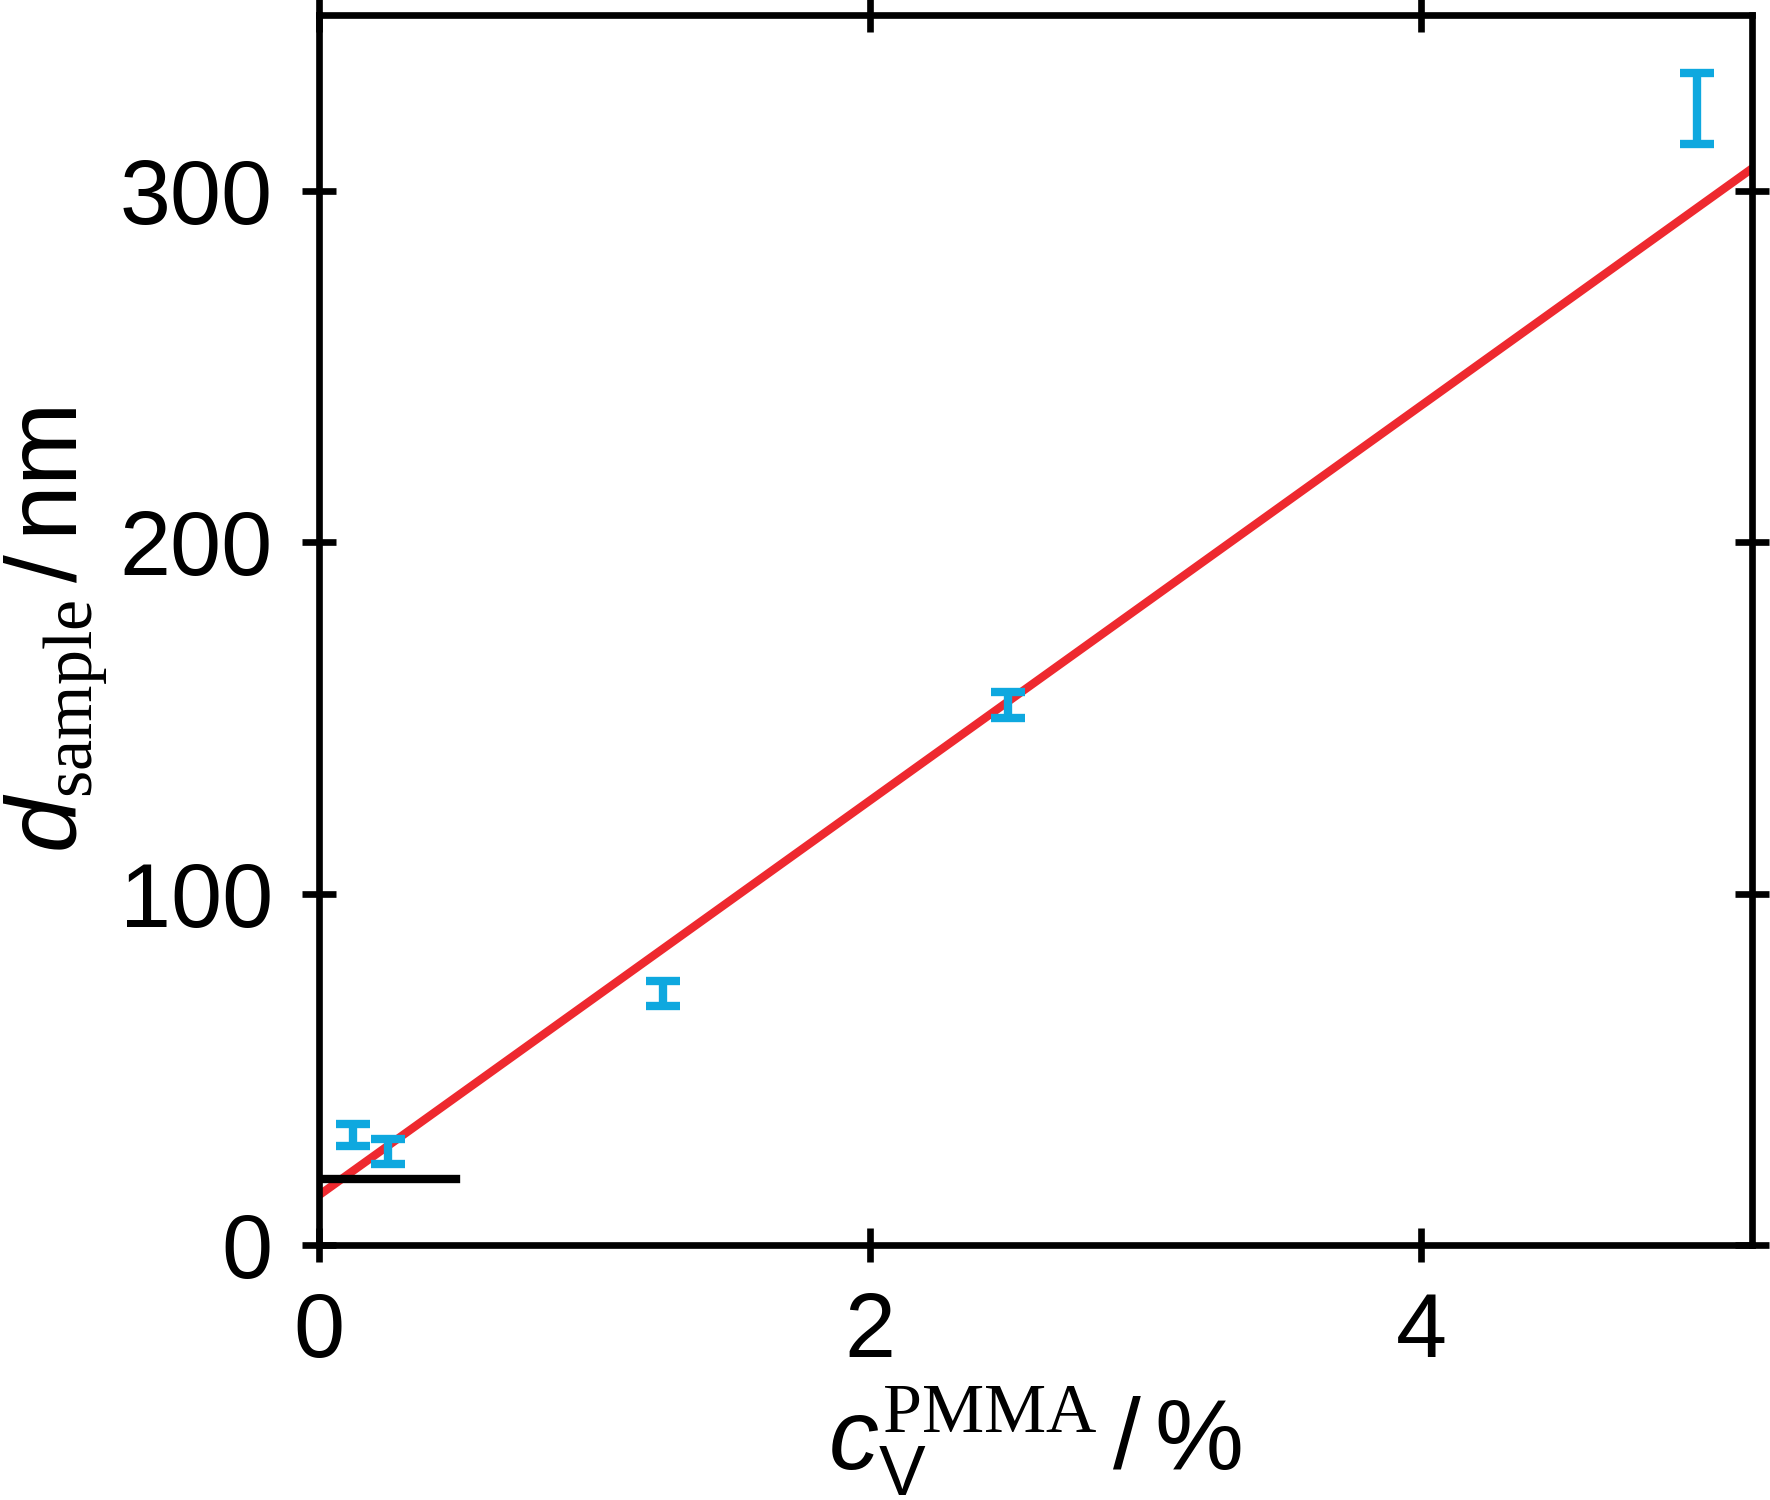
\includegraphics{doublelayers_SEM_Thickness}
    \caption{\label{fig:doublelayers:layers:xs}Cross-sectional SEM micrographs of DL-0.125\% (upper left), DL-0.25\% (upper right), DL-1.25\% (center left), DL-2.5\% (center right) and DL-5\% (lower left). The sample thickness with respect to the PMMA concentration used during spin coating is shown in the lower right. }
  \end{figure}

\end{document}